\documentclass[Project Report]{article}
\usepackage{graphicx}
\usepackage{fancyhdr}
\usepackage{sectsty}
\usepackage{url}
\usepackage[margin=1in]{geometry}



% \author{Ryan Ayotte, SN: 101073548}
% \title{COMP3005 Project}
\pagestyle{fancy}
\lhead{COMP3005 Final Project Report}
\rhead{Ryan Ayotte SN: 101073548}
\sectionfont{\fontsize{12}{15}\selectfont}

\begin{document}

\section{Conceptual Design}
{\centering 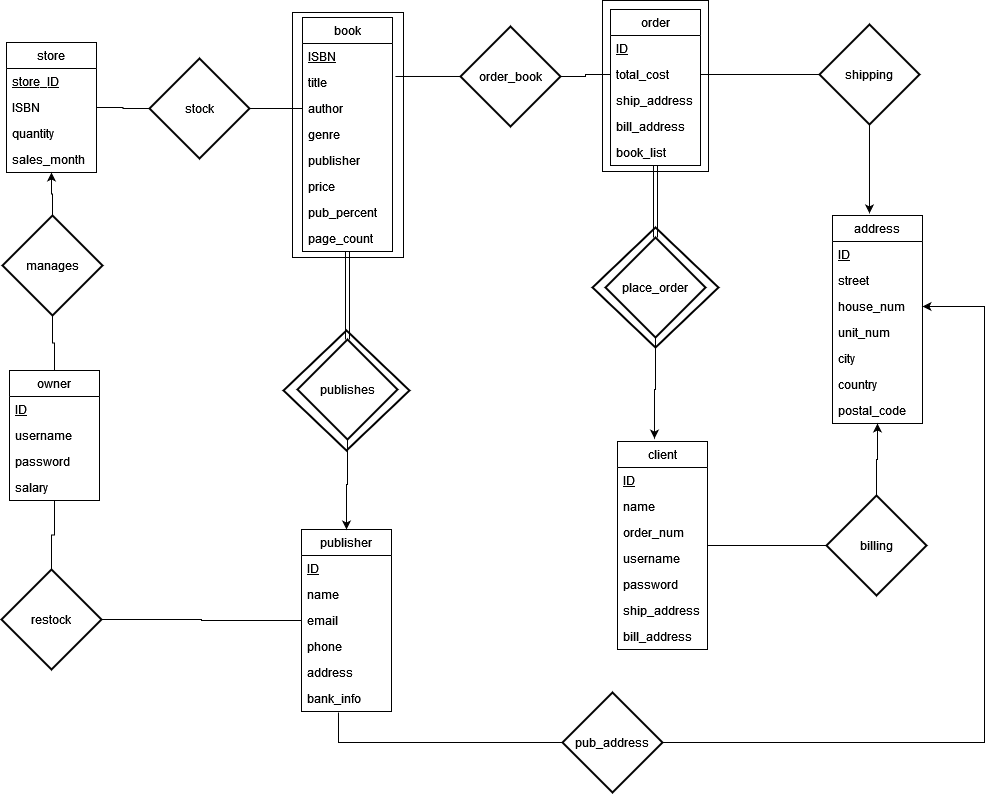
\includegraphics[width=\textwidth]{ER_Diagram.png}}
\begin{itemize}
    \item store: A store is managed by an owner and keeps track of the current stock of each book as well as the sales made for each month
    \item owner: An owner can manage the inventory of the store as well as purchase more from the publishers should stock be running low
    \item book: A book has its stock managed through the store and is published by publishers who also get a percetage of the book's sale. The assumption for a book to exist is that it is first published and provided by the publisher. Books can also be added to orders by the client to be purchased
    \item publisher: A publisher publishes books and provides them to the store owner for their store. They peovide their banking information to receive their part of their book sale, and they have an address they can be reached at
    \item order: An order can be made by a client to buy books from the store and have them sent to the provided shipping address. The assumption for an order to exist is that a client must already exist who have placed the order.
    \item client: A client, who is registered with the store, can place an order of books to be sent to a provided shipping address, paied bia their billing address.
    \item address: An address specifies the location for either a publisher, a client, or a client's billing info
\end{itemize}

\section{Reduction to Relation Schemas}
\begin{itemize}
    \item store: (\underline{store\_id}, ISBN, quantity, sales\_month)
    \item owner: (\underline{ID}, username, password, salary)
    \item book: (\underline{ISBN}, title, author, genre, publisher, price, pub\_percent, page\_count)
    \item publisher: (\underline{ID}, name, email, phone, address, bank\_info)
    \item order: (\underline{ID}, total\_cost, ship\_address, bill\_address, book\_list)
    \item client: (\underline{ID}, name, username, password, ship\_address, bill\_address)
    \item address: (\underline{ID}, street, house\_num, unit\_num, city, country, postal\_code)
    \item stock: (\underline{ISBN}, \underline{store\_id})
    \item manages: (\underline{owner\_id}, \underline{store\_id}, ISBN, quantity)
    \item restock: (\underline{owner\_id}, \underline{pub\_id})
    \item publishes: (\underline{ISBN}, \underline{pub\_id}, pub\_percent, bank\_info)
    \item order\_book: (\underline{ISBN}, \underline{order\_id})
    \item place\_order: (\underline{client\_id}, \underline{order\_id}, ship\_address, bill\_address)
    \item pub\_address: (\underline{add\_id}, \underline{pub\_id})
    \item shipping: (\underline{order\_id}, \underline{address\_id})
    \item billing: (\underline{client\_id}, \underline{address\_id})
\end{itemize}

\section{Normalization of Relation Schemas}
Unsure what to put here at the moment......

\section{Database Schema Design}
{\centering 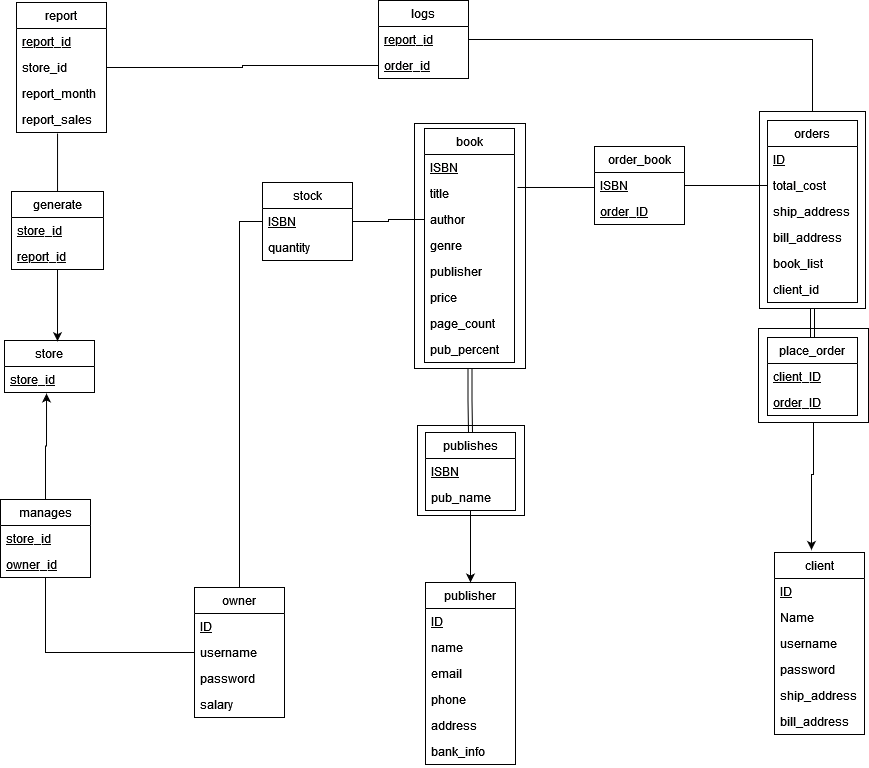
\includegraphics[width=\textwidth]{Schema_Diagram.png}}

\section{Implementation}
Currently incomplete

\section{Bonus Features}
No bonus features in project currently

\section{GitHub Repository}
\url{https://github.com/rayotte/COMP_3005_Project}

\section{Appendix I (Availability)}
Exempted from demonstrations based on prior conversation with professor Roby

\end{document}